\textbf{Setup and Dataset.}
To capture realistic discharge statistics under dynamic flight profiles, we collected an extensive dataset using single-cell LiPo batteries from a Crazyflie 2.1 fleet.
Rather than relying on static bench tests, we compiled approximately 3 hours of active flight data across 200 distinct sorties, incorporating both standard demonstrations~\cite{ullah2026nanobench} and multi-sortie waypoint navigation tasks.
Crucially, the data was sourced from 14 individual battery cells, explicitly capturing the heterogeneous voltage drop characteristics encountered in physical deployments.
We fit a physically parameterized load-voltage proxy model to this dataset, evaluating the calibration performance using a strict held-out testing approach for each independent cell.

\textbf{Results.}
We evaluate whether adaptive conformal inference reliably maintains the one-sided energy bounds below the target violation level ($\delta=0.10$). 
As illustrated in Fig.~\ref{fig:fig3} (left), the adaptive framework successfully drives the empirical violation frequency below the target threshold over sequential calibration rounds.
Furthermore, when evaluated across all 14 individual battery cells under distribution shift, our adaptive method robustly bounds the error (Fig.~\ref{fig:fig3} (right)). 
In contrast, a standard fixed-quantile baseline fails to adapt to cell-specific degradation, resulting in uncalibrated bound violations with a mean of $0.116$ and a standard deviation of $0.114$. 
These comparative results confirm that our calibration layer effectively absorbs usage-induced discrepancies, producing a statistically sound energy-sufficiency margin to serve as a trustworthy precedence cue.

\begin{figure}[t!]
\centering
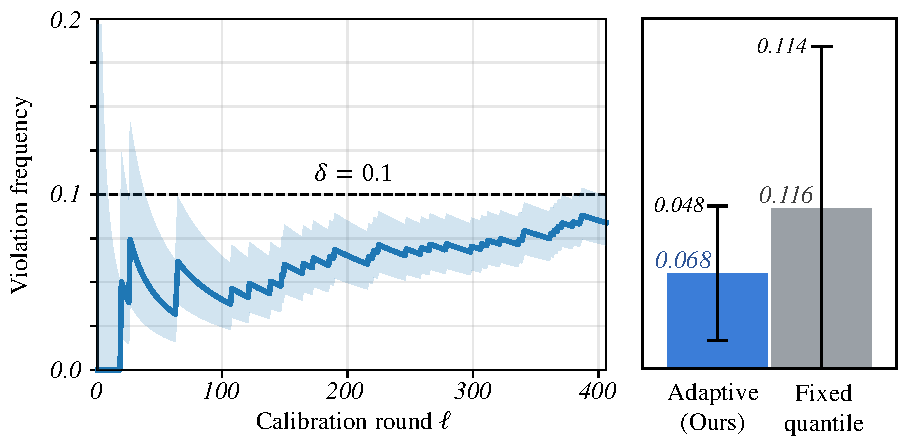
\includegraphics[width=\columnwidth]{Figures/fig3.pdf}
\caption{Battery calibration performance. \textbf{(Left)} The running violation frequency converges below the target $\delta=0.1$. \textbf{(Right)} Our adaptive method successfully bounds errors across 14 cells (mean $0.068$, std $0.048$), outperforming the fixed-quantile baseline.
}
\vspace{-10pt}
\label{fig:fig3}
\end{figure}